\section{State of the Art: FCA2VEC\label{sec:fca2vec}}

Binary FCs are binary tables. There exist a wide variety of \textit{rank lowering} methods to represent such tables, like \textit{latent semantic analysis} in NLP.
The resulting representation is usually a pair of sets of vectors, one for the rows and one for the columns of the table.
However, such methods do not take into account the properties manipulated by FCA, such as the closure operator or the formal concepts.

To our knowledge, the only embedding framework specialized for FCs and based on FCA is FCA2VEC~\cite{fca2vec:2019:durrschnabel} by  Dürrschnabel \etal{}.
We explain the major aspects of their approach in this section. For further detail, see the original article.
In \cref{sec:fca2vec-o2v} and \cref{sec:fca2vec-c2v}, we describe the embedding architectures based on FCA's closure operator proposed in~\cite{fca2vec:2019:durrschnabel}, namely \textit{object2vec}, \textit{attribute2vec}, and \textit{closure2vec}.
Finally, we describe in \cref{sec:fca2vec-evaluation} the methods used in the article to evaluate {object2vec} and {attribute2vec}.
Note that all FCA2VEC models are designed to build embeddings of small dimensions (2 or 3 elements only).

\subsection{{Object2vec} and {Attribute2vec}}\label{sec:fca2vec-o2v}
\textit{Object2vec} and \textit{attribute2vec} are proposed in FCA2VEC to provide embeddings of objects and attributes using respectively the extents and the intents.
They are based on the idea \blockcquote{fca2vec:2019:durrschnabel}{to interpret two objects to be more close to each other if they are included in more concept extents together.}

Based on this principle, the authors adapt the \textit{word2vec}~\cite{word2vec:2013:mikolov} distributional word embedding framework.
{Word2vec} learns to associate a word with the words it appears with often, by learning to predict either the context of a word given the word (\textit{skip-gram} variant) or a word based on its context (\textit{CBoW} variant). This principle is schematized in \cref{fig:w2v}.
By interpreting the objects as words and the extents as sentences and applying {word2vec}, an object will be associated with objects often appearing in the same extent. The resulting model is called {object2vec}.
Similarly, {attribute2vec} is obtained by using attributes as words and intents as sentences. 

\begin{figure}
    \centering
    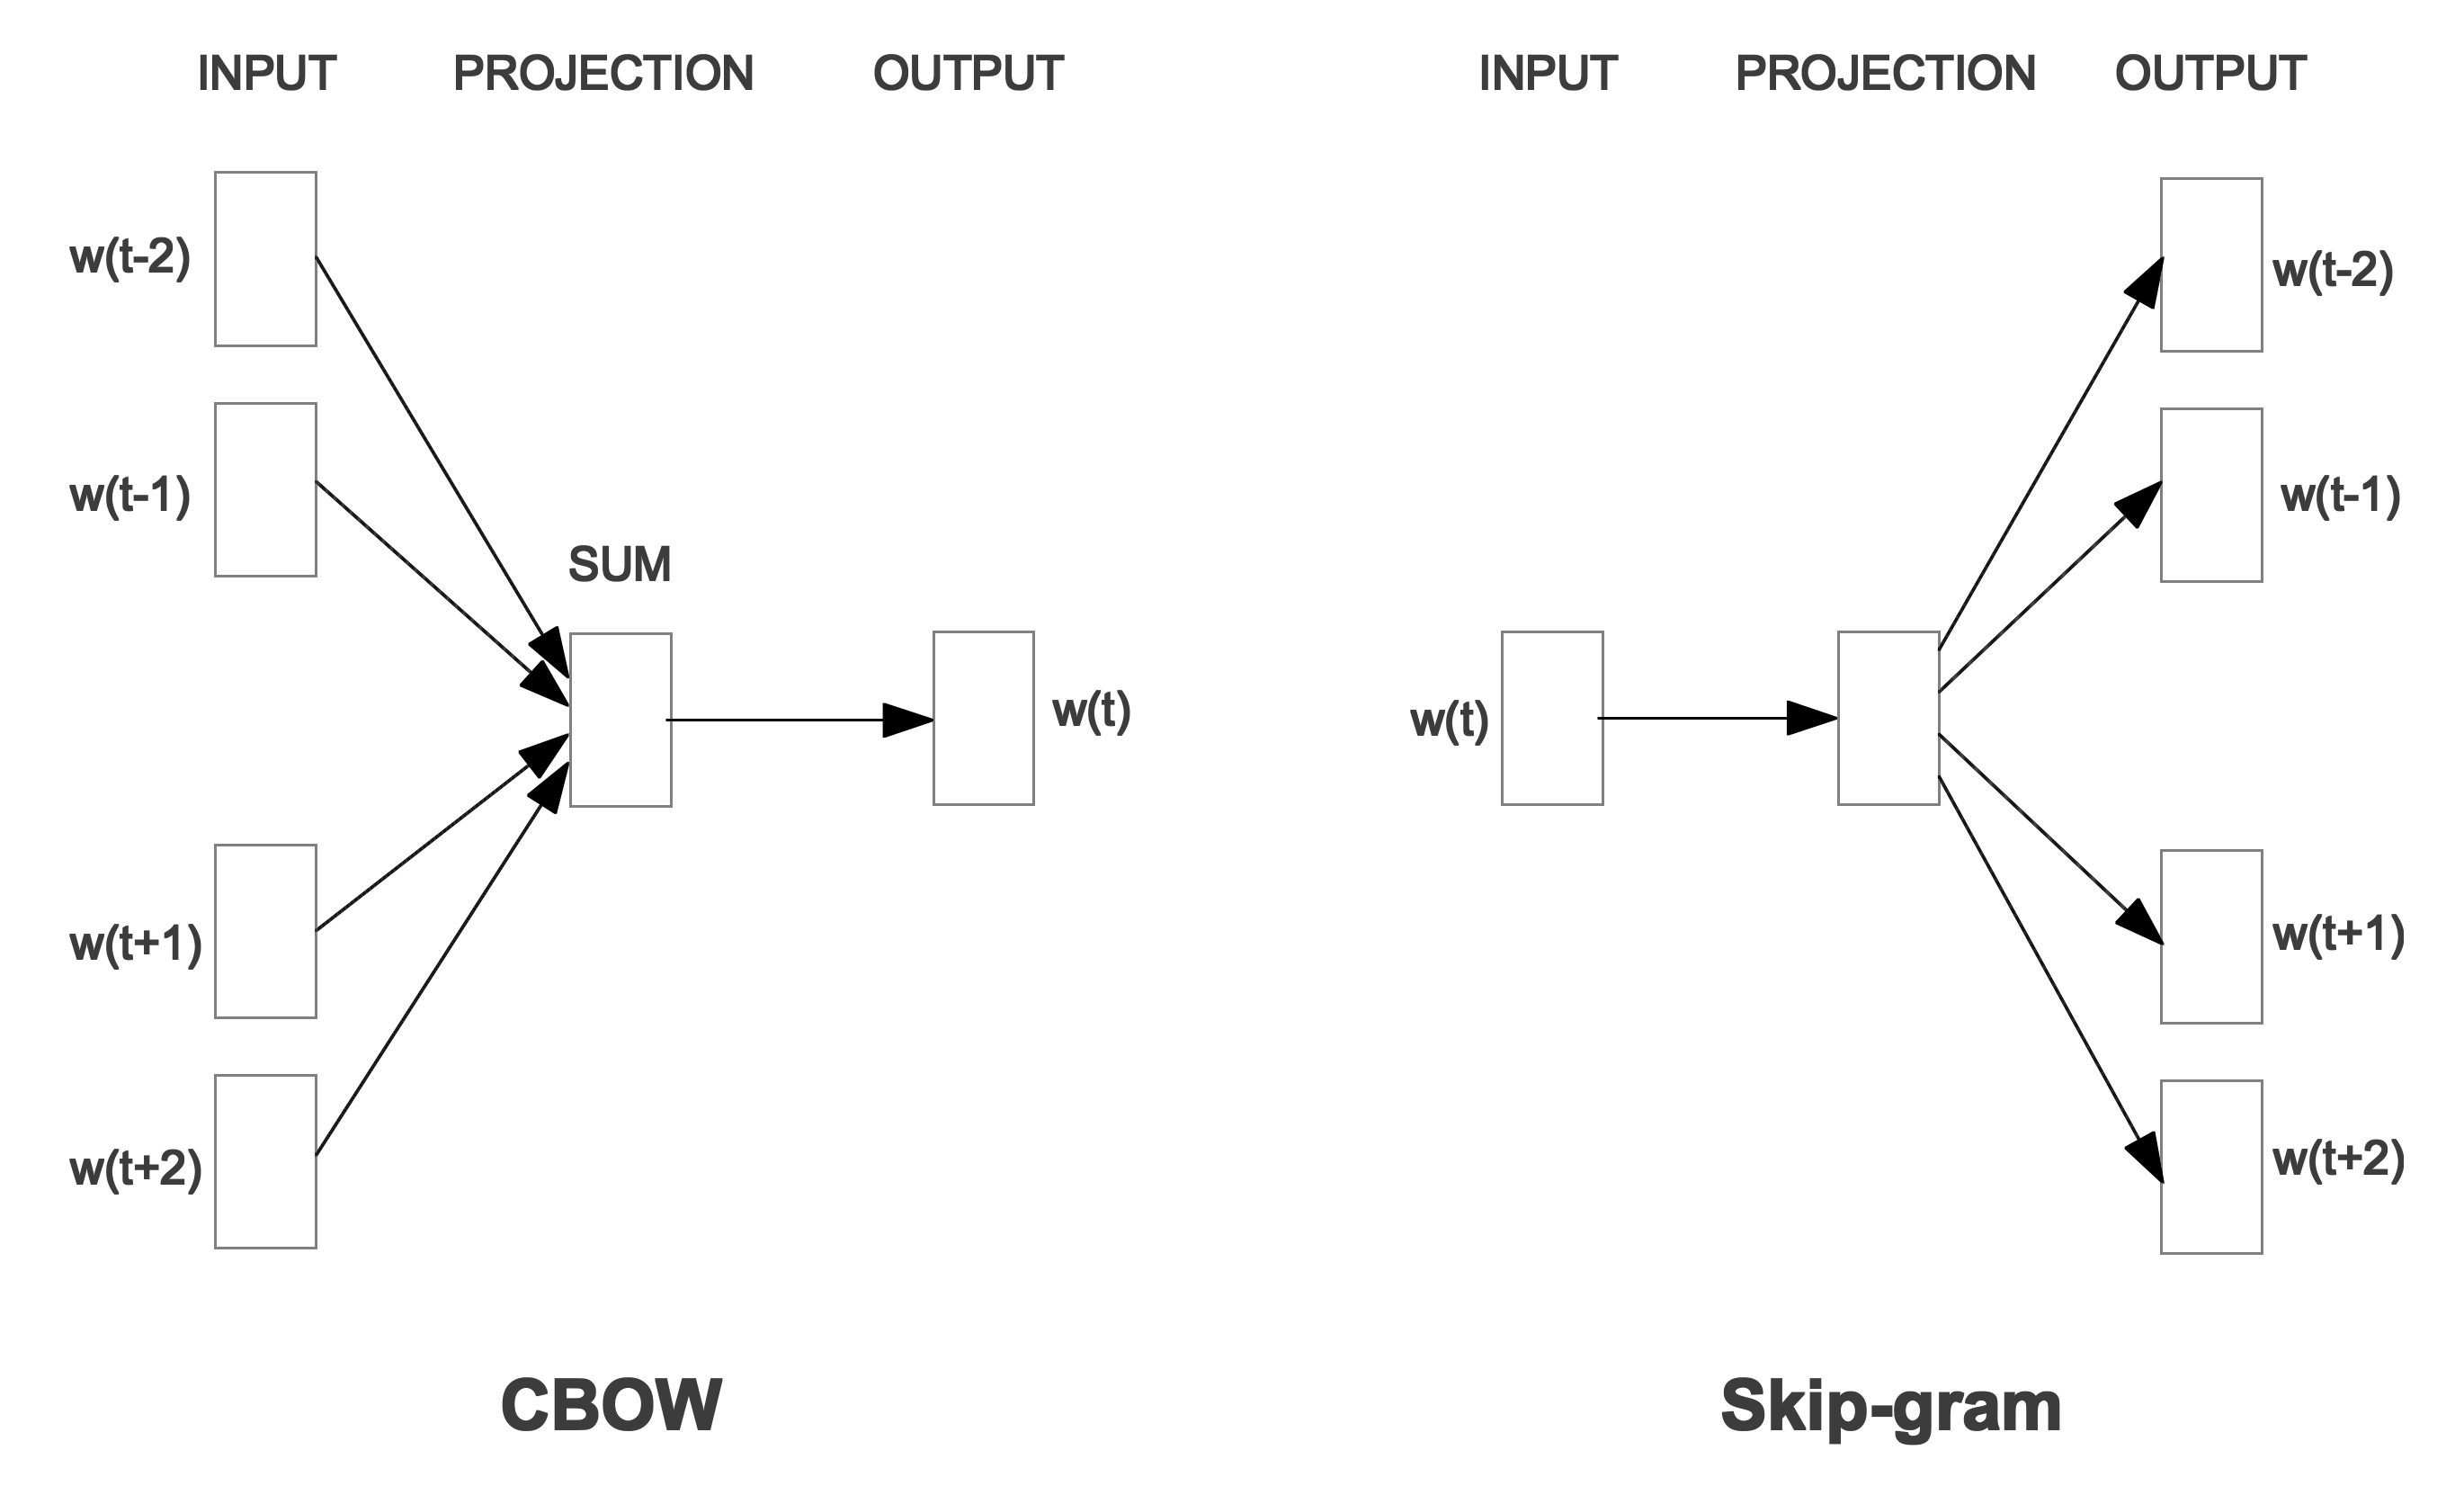
\includegraphics[width=.9\textwidth, height=5cm, keepaspectratio]{Figures/Ch2/word2vec.png}
    \caption{Continuous Bag of Words (CBoW) and skip-gram architectures from word2vec. Figure 1 from \cite{word2vec:2013:mikolov}.}
    \label{fig:w2v}
\end{figure}

The samples used to train {object2vec} are generated by taking, for each extent $e$, for each object $o_1\in e$, either:
\begin{itemize}
    \item all the pairs $\langle o_1, o_2 \rangle$ for all the other objects $o_2$ in the extent ($o_2 \in e/o_1$\footnote{As a reminder, $e/o_1$ stands for the set $e$ without the element $o_1$.\label{fn:e-less-o}}), for the {skip-gram} variant;
    \item the pair $\langle e/o_1, o_1 \rangle$, for the {CBoW} variant.
\end{itemize}
In practice, $o_1$ and $o_2$ are represented by their respective one-hot encoding, and $e/o_1$ is represented by the element-wise average vector of the one-hot encoding of its elements.

It is interesting to note that for an extent of size $|e| = 5$, 5 samples are generated for {CBoW}, while for {skip-gram} $5\times 4$ (2 among 5) samples are generated. For FCs with large amounts of objects and concepts, the number of samples used to train the {skip-gram} variant is explosively large using this method.

\subsection{Closure2vec}\label{sec:fca2vec-c2v}
\textit{Closure2vec} is proposed in FCA2VEC based on the result of~\cite{encoding:2007:rudolph}.
Rudolph demonstrates that for any closure operator on two sets $X$ and $Y$, there exists an MLP able to perfectly encode said closure operator.
The MLP of the closure operator from $X$ to $X$ has an input size of $|X|$, a first layer with $|Y|$ neurons and a second one with $|X|$ neurons.
This general result is applicable to FCA's closure operator, \eg, $\cdot''$ on the set of attributes can be encoded with a 2 layer MLP with an input size of $|A|$, a first layer with $|O|$ neurons and a second one with $|A|$ neurons.
Such a model, once defined, can be learned using deep learning algorithms.

{Closure2vec} is designed to take two sets of attributes (for example, two objects) and compute an embedding for each of them.
It is then trained to match the \textit{closure Hamming distance} (see \cref{def:chd}) between the two sets of attributes to the distance between the corresponding embeddings. The distance between the embeddings is computed using either the Euclidian or the cosine distance.
In practice, {closure2vec} uses a 2 layer MLP as defined in~\cite{encoding:2007:rudolph}, with an additional feed-forward layer that computes a 2- or 3-dimensional embedding vector.

\begin{definition}\label{def:chd}
The \emph{closure Hamming distance} (CHD) between two sets of attributes is the \emph{Hamming distance} between the binary representation of respective closures of the two sets of attributes. In other words, it is the number of modifications necessary to go from one closure to the other.
Two attribute sets are called \emph{equivalent} if they have the same closure, so if their CHD is 0.
\end{definition}

{Closure2vec} is trained on randomly sampled pairs of sets of attributes, with the sets in a pair differing by exactly one attribute.

\subsection{Evaluation}\label{sec:fca2vec-evaluation}
In this subsection, we describe the evaluation processes used to evaluate {attribute2vec} and {object2vec}.
For the evaluation, the authors use real-world datasets and tasks using the embeddings.

%For \textit{closure2vec}, the authors evaluate the CHD between the intents of the concepts of the wiki44k and the Mushroom datasets.

\begin{table}
    \centering
    \begin{tabular}{lllll}
    \toprule
    Dataset & \# Objects & \# Attributes & Density & \# Concepts\\
    \midrule
    ICFCA$^\star$ & 263 & 8442 & 0.005 & 680 \\
    Wiki44k & 45021 & 101 & 0.04 & 21923\\
    \bottomrule
    \end{tabular}
    \caption{Descriptive statistics on ICFCA$^\star$ and wiki44k, the datasets used to evaluate {object2vec} and {attribute2vec}. Table 1 from~\cite{fca2vec:2019:durrschnabel}.}
    \label{tab:fca2vec-datasets}
\end{table}

\subsubsection{Attribute Clustering for Attribute2vec\label{sec:fca2vec-clustering}}
The performance of \textit{attribute2vec} is evaluated through an attribute clustering task.
The \textit{wiki44k} dataset\footnote{Available at \url{http://people.mpi-inf.mpg.de/~gadelrab/RuLES/}.} is used for this experiment. 
Wiki44k is a knowledge graph (KG) where \textit{entities} (the nodes) are put in relation using \textit{statements} (directed labeled edges) labeled with \textit{properties} (edge labels).
The corresponding FC uses the entities as objects and property names as attributes. An object $o_i$ and an attribute $a_j$ are related by the incidence relation if entity $o_i$ appears in a statement labeled with property $a_j$.
As the authors of~\cite{fca2vec:2019:durrschnabel} mention, wiki44k is sparse for an FC, with a density of 0.04.

The canonical base of wiki44k is used for the attribute clustering task of~\cite{fca2vec:2019:durrschnabel}.
A canonical base can be seen as a minimal set of implications (of the form $X\rightarrow Y$, with $X, Y\in A$) which is sufficient to describe all the valid implications of a lattice.
An implication $X\rightarrow Y$ is valid if $Y$ appears every time $X$ does, \ie, if we have $X$, we always have $Y$.
Hanika, one of the authors of~\cite{fca2vec:2019:durrschnabel}, explains in~\cite{wiki44k-tr:2019:hanika} the interest of studying the canonical base of the FC of wiki44k. For further detail on the canonical base see, \eg, \cite{canonical:2016:karell,wiki44k-tr:2019:hanika}.

The attribute clustering task consists in clustering attribute embeddings using a simple clustering algorithm (k-means).
The performance is measured by taking the rate of \textit{intra-cluster} implications, \ie, implications from the canonical base which are \blockcquote{fca2vec:2019:durrschnabel}{completely contained in one cluster}. An implication $X \rightarrow Y$ is called \textit{intra-cluster} if there is a cluster $K$ such that $X \cup Y \in K$.
Two baselines are used: \textit{(i)} a random clustering, obtained by generating random clusters with similar sizes as ones obtained by {attribute2vec}, and \textit{(ii)} a naive clustering, obtained by clustering a naive representation of the attributes. For an attribute $a$, this naive representation is the binary encoding of $a'$, the set of objects having the attribute $a$.

The performance reported in~\cite{fca2vec:2019:durrschnabel} is shown in \cref{tab:fca2vec-a2v-perf}.
The performance of {attribute2vec}'s CBow variant is lower than the random baseline, so the corresponding results are not reported by~\cite{fca2vec:2019:durrschnabel}. 
{Attribute2vec} skip-gram outperforms the two baselines, which could be expected given the training objective of attribute2vec.
Indeed, attribute2vec is trained to bring together attributes often appearing in the same intents, and implications describe sets of attributes appearing together in the dataset.

\begin{table}
    \centering
    \begin{tabular}{rllll}
    \toprule
    Emb. size & Model & $k = 2$ & $k = 5$ & $k = 10$ \\
    \midrule
    & Naive & $0.0158\pm0.0000$ & $0.0055\pm0.0042$ & $0.0035\pm0.0002$\\
    \midrule
    \multirow{2}{*}{2} & Random & $0.0534\pm0.0412$ & $0.0084\pm0.0088$ & $0.0010\pm0.0007$ \\
    & a2v-SG & $0.1608\pm0.0031$ & $0.0703\pm0.0122$ & $0.0069\pm0.0004$ \\
    \midrule
    \multirow{2}{*}{3} & Random  & $0.0219\pm0.0107$ & $0.0036\pm0.0027$ & $0.0007\pm0.0004$ \\
    & a2v-SG & $0.3217\pm0.0005$ & $0.1038\pm0.0218$ & $0.0080\pm0.0001$ \\
    \bottomrule
    \end{tabular}
    \caption{Rate of intra-cluster implication with the {attribute2vec} skip-gram variant (\textit{a2v-SG}) and the {naive} and {random} baselines, for embeddings of size 2 and 3, for $k=2$, $5$ and $10$ clusters, for 20 repetitions of the evaluation experiment (mean $\pm$ std.). Table 3 from~\cite{fca2vec:2019:durrschnabel}.}
    \label{tab:fca2vec-a2v-perf}
\end{table}

% Dataset:
% - wiki44k (http://people.mpi-inf.mpg.de/~gadelrab/RuLES/), from "rule learning from knowledge graphs guided by embedding models", adapted by "Discovering Implicational Knowledge in Wikidata"
% - wiki44k cannonical base for score computation

% > For comparison, we have also included the data set wiki44k as provided by [15], a small subset of simple statements extracted from a Wikidata dump from December 2014. Meanwhile, though, the usage of some properties on Wiki-data has changed, and, in particular, eight properties usedin this data set have since been deleted on Wikidata. Hence, we have also generated wiki44k-tr,where these properties have been replaced by their modern equivalents:
% - P7(“brother”), P9 (“sister”): replaced by P3373 (“sibling”)
% - P45 (“grandparent”): replaced by P1038 (“relative”) with a P1039 (“type of kinship”) qualifier with value Q167918 (“grandparent”)
% - P70 (“order”): replaced by P171 (“parent taxon”), where the object gets an additional P105 (“taxon rank”) statementwith value Q36602 (“order”),
% - P71 (“family”): replaced by P171 (“parent taxon”);where the object gets an additional P105 (“taxon rank”) statement with valueQ35409 (“family”),
% - P107 (“main type GND”), P132 (“administrative entity”):replaced by P31 (“instance of”), and
% - P133 (“language family”): replaced by P279 (“subclass of”).
% Both data sets were converted to JSON formatand then processed analogously to the other data sets. Data sets wiki44k-2018 and wiki44k-2018-tr are subsets of the 2018 dump obtained by dropping all items and properties (and statements connecting those) not appearing in wiki44k and wiki44k-tr, respectively.

% properties

% Their pipeline:
% 1. Applying attribute2vec on wiki44k (lr=1.0, ~5 epochs)
% 2. K-means clustering of embeddings (Sklearn, k-means++, the default), with k=2, k=5, k=10
% 3. Intra-cluster implications:
% %    > An implication drawn from the canonical base, i.e., A→B ∈ L, is called intra-cluster if there is some c∈C such that A∪B⊆c. The canonical base of wiki44k has the size 7040.For a clustering C we compute the ratio of intra-cluster implications.
% %    > Definition 11 (Canonical basis [30]). The canonical basis Σ_{cb} on S is defined by:
% %    Σ_{cb} = {B → φ(B) \ B : B ⊆ S is a pseudo-closed set of φ}
% %    where a subset B of S is pseudo-closed when B is not closed (i.e. B 6= φ(B)), and φ(B') ⊂ B for every pseudo-closed B' ⊂ B.

% 4. repeat 1/2/3 20 times
% 5. baseline:
%     - random clustering of attribute set
%     - "naive" clustering: attribute m represented by one-hot encoding of objects, then k-means

% Canonical basis from lattice:
% 1. before all: 
%     The canonical basis cannot be directly obtained with a lattice L as input.
% %    One needs to compute an IS Σ representing L before computing the canonical basis of Σ with the previous treatment.
% %    In [49], the following IS Σ defined on J_{L} is stated to characterize L:
% %        Σ = {J_{x} + j → J_{xVj} : x ∈ L, j ∈ JL , j 6≤ x and J_{x} + j not closed}
% %2. First, apply the right maximal transformation by replacing the conclusion of each rule X → Y by φ(X) \ X;
% 3.
% 4.



\subsubsection{Link Prediction for Object2vec\label{sec:fca2vec-link}}
A link prediction task is used to evaluate \textit{object2vec}.
The \textit{object2vec} model is applied on ICFCA$^\star$\footnote{ICFCA$^\star$ is available at the \textit{conexp-clj} repository: \url{https://github.com/tomhanika/conexp-clj}.}, a dataset of co-authorship in the FCA community. Descriptive statistics on the dataset are reported in \cref{tab:fca2vec-datasets}.
It is interesting to note that the dataset used is very sparse for an FC, with a density of 0.005, almost 10 times lower than the already sparse of wiki44k.
In the co-authorship graph, two authors have an edge between them if they are co-authors of an article.
The FC of this dataset uses authors as objects, papers as attributes, and the incidence relation is the authorship of a paper by an author.
The dataset is split in two: all the papers published strictly before 2016 are used to train the embedding model (training set), and all the papers from January 2016 to August 2019 are used to evaluate the performance of the model (evaluation set). Only the articles written by authors appearing in the training set are kept for the evaluation set.

To evaluate the performance, the author (or object) embeddings are generated on the whole dataset.
Co-authorship embeddings are then computed by taking the element-wise product of two randomly sampled author embeddings.
Half of the generated embeddings correspond to actual co-authorship in the dataset and are called positive samples.
The other half is made of negative samples, in other words, pairs of authors who are never co-authors in the dataset.
A basic classifier (logistic regression) is trained on the training set to predict if the co-authorship relation described by the corresponding embedding is true or not.
The performance of this classifier is then evaluated on the test set.
As a baseline, the authors of~\cite{fca2vec:2019:durrschnabel} use the node embeddings computed on the co-authorship graph by \textit{node2vec}~\cite{node2vec:2016:grover}, a graph embedding method similar to DeepWalk (see \cref{sec:soa-node}).

The performance reported in~\cite{fca2vec:2019:durrschnabel} is shown in \cref{tab:fca2vec-o2v-perf}.
For this task, {object2vec} outperforms {node2vec} by at least 5\% on each score, for both sizes of embedding.
The CBoW variant slightly outperforms the skip-gram one.

\begin{table}
    \centering
    \begin{tabular}{rllll}
    \toprule
    Emb. size & Model & Recall & Precision & F1\\
    \midrule
    \multirow{3}{*}{2} & node2vec & $0.56\pm0.14$ & $0.60\pm0.07$ & $0.57\pm0.09$ \\
    & o2v-SG & $0.66\pm0.08$ & $0.65\pm0.03$ & $0.65\pm0.05$ \\
    & o2v-CBoW & $0.68\pm0.09$ & $0.64\pm0.04$ & $0.66\pm0.06$ \\
    \midrule
    \multirow{3}{*}{3} & node2vec & $0.60\pm0.15$ & $0.56\pm0.08$ & $0.58\pm0.10$ \\
    & o2v-SG & $0.70\pm0.08$ & $0.62\pm0.04$ & $0.66\pm0.06$ \\
    & o2v-CBoW & $0.73\pm0.07$ & $0.65\pm0.06$ & $0.69\pm0.06$ \\
    \bottomrule
    \end{tabular}
    \caption{Performance of the two \textit{object2vec} variants and the \textit{node2vec} baseline, for embeddings of size 2 and 3, for 30 repetitions of the evaluation experiment (mean $\pm$ std.). \textit{o2v-SG} stands for the skip-gram and \textit{o2v-CBoW} for the CBoW variant. Table 2 from~\cite{fca2vec:2019:durrschnabel}.}
    \label{tab:fca2vec-o2v-perf}
\end{table}

% > Link Prediction using Object2Vec

% Dataset:
% - ICFCA
% - "object" is author
% - "attribute" is "all publications of these authors" (p13, last §)
% - "link" is co-authorship edge between authors
% - train on < 2016-01-01 ~> 1278 examples, 50% negative
%     positives are edges (or pairs of nodes) without an edge connecting them < 2016-01-01
%     negatives are two randomly picked nodes without an edge connecting them (regardless of the date)
% - predict links in [2016-01-01; 2019-08-01] ~> 84 examples, 50% negative
%     positives are edges (or pairs of nodes) without an edge connecting them [2016-01-01; 2019-08-01]
%     negatives are two randomly picked nodes without an edge connecting them (regardless of the date)

% Their pipeline:
% 1. Applying object2vec (lr=1.0, linear decrease, 200 epochs, repeat 30 times)
% 2. Apply node2vec
% 3. Edge vector generation, componentwise product of two node vectors
% 4. Classification (Logistic regression, Sklearn, C param determined by grid search in [1e-3, 1e-2, 1e-1, 1e0, 1e1, 1e2])






